% Copyright (c) 2008-2009 solvethis
% Copyright (c) 2010-2016 Casper Ti. Vector
% Public domain.
%
% 使用前请先仔细阅读 pkuthss 和 biblatex-caspervector 的文档,
% 特别是其中的 FAQ 部分和用红色强调的部分。
% 两者可在终端/命令提示符中用
%   texdoc pkuthss
%   texdoc biblatex-caspervector
% 调出。

% 采用了自定义的(包括大小写不同于原文件的)字体文件名,
% 并改动 ctex.cfg 等配置文件的用户请自行加入 nofonts 选项;
% 其它用户不用加入 nofonts 选项,加入之后反而会产生错误。
\documentclass[UTF8]{pkuthss}

% 使用 biblatex 排版参考文献,并规定其格式(详见 biblatex-caspervector 的文档)。
% 这里按照英文文献在前,中文文献在后排序(“sorting = ecnty”);
% 若需按照中文文献在前,英文文献在后排序,请设置“sorting = centy”;
% 若需按照引用顺序排序,请设置“sorting = none”。
% 若需在排序中实现更复杂的需求,请参考 biblatex-caspervector 的文档。
\usepackage[backend = biber, style = caspervector, utf8, sorting = ecnty]{biblatex}

% 按学校要求设定参考文献列表中的条目之内及之间的距离。
\setlength{\bibitemsep}{3bp}
% 对于 linespread 值的计算过程有兴趣的同学可以参考 pkuthss.cls。
\renewcommand*{\bibfont}{\zihao{5}\linespread{1.27}\selectfont}

% 设定文档的基本信息。
\pkuthssinfo{
	cthesisname = {硕士研究生学位论文}, ethesisname = {Doctor Thesis},
	ctitle = {基于谓词频谱的缺陷定位工具的设计与实现}, 
	etitle = {The Design and Implementation of a Fault Localization Tool Based on Predicate Spectrum},
	cauthor = {王然},
	eauthor = {Ran Wang},
	studentid = {1501214409},
	date = {二零一八年五月},
	school = {信息科学技术学院},
	cmajor = {计算机软件与理论}, emajor = {Computer Software and Theory},
	direction = {软件开发环境},
	cmentor = {郝丹副教授}, ementor = {Dan Hao, Yingfei Xiong and Lu Zhang},
	ckeywords = {缺陷定位,程序调试,机器学习}, ekeywords = {Fault localization, Program debugging, Machine learning},
	cmentorsub = {熊英飞研究员,张路教授},
}
% 载入参考文献数据库(注意不要省略“.bib”)。
\addbibresource{thesis.bib}

% 普通用户可删除此段,并相应地删除 chap/*.tex 中的
% “\pkuthssffaq % 中文测试文字。”一行。
\usepackage{color}
% \def\pkuthssffaq{%
% 	\emph{\textcolor{red}{pkuthss 文档模版最常见问题:}}

% 	\texttt{\string\cite}、\texttt{\string\parencite} %
% 	和 \texttt{\string\supercite} 三个命令分别产生%
% 	未格式化的、带方括号的和上标且带方括号的引用标记:%
% 	\cite{test-en},\parencite{test-zh}、\supercite{test-en, test-zh}。

% 	若要避免章末空白页,请在调用 pkuthss 文档类时加入 \texttt{openany} 选项。

% 	如果编译时不出参考文献,
% 	请参考 \texttt{texdoc pkuthss}“问题及其解决”一章
% 	“上游宏包可能引起的问题”一节中关于 biber 的说明。
% }

\newcommand\todo[1]{\textcolor{red}{\{TODO:#1\}}}
\newcommand\mycode[1]{{\small\ttfamily #1}}
\newcommand\toolname{基于谓词频谱的缺陷定位工具}
\usepackage{hyperref}

\usepackage{listings}
\usepackage{multirow}
\usepackage{array}
\lstset{
    numbers=left, 
    numberstyle=\tiny,
    keywordstyle= \color{ blue!70},
    commentstyle= \color{red!50!green!50!blue!50}, 
    frame=shadowbox, % 阴影效果
    rulesepcolor= \color{ red!20!green!20!blue!20},
    basicstyle=\small\ttfamily,
    breaklines
} 

\newcounter{finding}
\newcommand{\finding}[1]{\refstepcounter{finding}
    \vspace{3.0pt}
    \fbox{
        \parbox{0.9\columnwidth}{
            \textbf{发现 \arabic{finding}. } \emph{#1}
        }
    }
    \vspace{3.0pt}
}

\begin{document}
	% 以下为正文之前的部分,默认不进行章节编号。
	\frontmatter
	% 此后到下一 \pagestyle 命令之前不排版页眉或页脚。
	\pagestyle{empty}
	% 自动生成封面。
	\maketitle
	% 版权声明。封面要求单面打印,故需新开右页。
	\cleardoublepage
	\include{chap/copyright}

	% 此后到下一 \pagestyle 命令之前正常排版页眉和页脚。
	\cleardoublepage
	\pagestyle{plain}
	% 重置页码计数器,用大写罗马数字排版此部分页码。
	\setcounter{page}{0}
	\pagenumbering{Roman}
	% 中英文摘要。
	% Copyright (c) 2014,2016 Casper Ti. Vector
% Public domain.

\begin{cabstract}

程序调试是一个耗费时间的任务,已经有很多研究者提出了各种不同的自动缺陷定位技术去减轻手动调试的负担。
在这些自动缺陷定位技术中,基于频谱的缺陷定位和基于状态覆盖的缺陷定位是两中比较常用的缺陷定位技术。
这两种技术都是在执行时收集一些统计信息。
这两种技术存在一些相似之处,但是两种技术一直单独地发展,而它们的结合也一直没有被系统地讨论过。

本文对基于频谱的缺陷定位和基于状态覆盖的缺陷定位技术的结合进行了系统的实证研究,
并且提出一种基于机器学习的谓词预测的方法帮助缺陷定位。
本文构建了一个两种技术的统一模型,并在这个模型上系统地探索了四种变体:
不同粒度的数据收集、不同的怀疑度公式、不同的怀疑度结合方式、不同的谓词。
此外,本文还提出了一个基于机器学习的谓词预测模型,来完善基于状态覆盖的缺陷定位原有的预定义谓词。

本文的研究得到了很多结论。
第一,更细粒度的数据收集的效果远远好于粗粒度的数据收集,并且只需要花费稍微多一点的执行时间。
第二,把基于频谱的缺陷定位公式应用在基于状态覆盖的缺陷定位的预定义谓词上,其效果反而好于原有的基于状态覆盖的缺陷定位的公式。
第三,一个基于频谱的缺陷定位和基于状态覆盖的缺陷定位的线性结合模型的效果比两者都更好。
第四,结合方法的效果大部分得益于分支谓词。
第五,预测的谓词在某些指标上获得了比预定义谓词更好的结果。预测谓词与预定义谓词具有互补性,两者结合后定位效果进一步提升。

\end{cabstract}

\begin{eabstract}

Program debugging is a time-consuming task,
and researchers have proposed different kinds of automatic fault localization techniques
to mitigate the burden of manual debugging.
Among these techniques, two popular families are spectrum-based fault localization
and statistical debugging,
both localizing faults by collecting statistical information at runtime.
Though the ideas are similar, the two families have been developed independently
and their combinations have not been systematically explored.

In this paper we perform a systematical empirical study on the combination of spectrum-based
fault localization and statistical debugging,
and we propose a predicate prediction technique based on machine learning to help to locate the faults.
We first build a unified model of the two techniques,
and systematically explores four types of variations:
different granularities of data collection,
different risk evaluation formulas, different ways of combining suspiciousness scores,
and different predicates.
Then we propose a machine-learning model to predict the predicates,
instead of using pre-defined predicates in statistical debugging.

The study leads to several findings.
First, fine-grained data collection significantly outperforms
coarse-grained data collection with a little more execution overhead.
Second, the risk evaluation formulas of spectrum-based fault localization
siginificantly outperforms that of statistical debugging when used in statistical debugging.
Third, a linear combination of spectrum-based fault localization and
statistical debugging outperforms both individual approaches.
Forth, most of the effectiveness of the combined approach contributed by a simple type of predicates:
branch conditions.
Fifth, the predicted predicates are better than pre-defined predicates in some metrics.
The predicated predicates and pre-defined predicates are complementary.
The combination of them has further improvement.
\end{eabstract}

% vim:ts=4:sw=4

	% 自动生成目录。
	\tableofcontents

	% 以下为正文部分,默认要进行章节编号。
	\mainmatter
	% 各章节。
	\chapter{引言}

本章主要介绍了自动缺陷定位的研究背景及其重要意义,然后阐述了本文的研究内容、主要贡献和论文结构。

\section{研究背景}

随着软件的发展,生活中越来越多的方面都与软件有着紧密的关系。
小到人们的日常出行、购物、餐饮等,大到航空航天、医药等领域,软件在人们的生活中扮演着重要的角色。
随着软件的应用领域的扩大,软件的复杂性上升,提升了软件缺陷的可能性。
软件缺陷可能会导致巨大的损失。
一个著名的被广泛引用的例子是海湾战争时,一颗导弹由于导航软件的精度缺陷而偏离了目标,导致28人死亡和100人受伤\parencite{Zou2015A}。
2002年,美国国家标准与技术研究院(NIST)发表的一篇报告\parencite{NIST2002The}显示,软件缺陷每年会导致约595亿美元的经济损失。\todo{每年这么多国内公司漏洞事件}
发现并修复软件缺陷,保障软件的高质量成为一项重要的任务。

\section{研究意义}

在发现软件缺陷之后,开发人员为了解决这个缺陷往往需要三步\parencite{Parnin2011Are}。
第一步,缺陷定位,需要找到程序中和这个缺陷有关的语句。
第二步,理解缺陷,明白为什么会发生缺陷。
第三步,修复缺陷,修改代码以让缺陷消失。
这三个步骤合起来就是调试的过程。缺陷定位作为调试的第一步,其完成速度和准确性对后面的步骤有着很大的影响。
在传统的开发环境当中,人们可以手动调试来定位缺陷,比如插入断点、打印日志信息等等。
在1989年Collofello等人就指出尝试去减少软件中的错误会花费50\%到80\%的开发和维护的精力\parencite{Collofello1989Evaluating}。
随着软件的复杂性的上升,手动地定位软件缺陷将会耗费更多开发者的时间和精力。
为了提高定位缺陷的速度,研究人员对自动化的缺陷定位展开了研究,并取得了巨大的进展\todo{cite}。
然而在2011年,Partin和Osro的一篇调查\parencite{Parnin2011Are}通过研究缺陷定位技术在实际应用场景下的效果,发现以往的评价指标并不能准确的反映缺陷定位技术在实际应用中的效果。
以往的缺陷定位技术是基于一系列关于开发人员会如何调试的假设,而这些假设在实际场景的某些情况下会失效。
自动化缺陷定位技术还有很大的发展空间。

\section{本文研究内容}

\section{本文主要贡献}

\section{论文结构}
	\chapter{相关工作}

本章将介绍自动缺陷定位、机器学习的相关工作和缺陷定位所使用的数据集以帮助更好理解本文的工作。

\section{自动缺陷定位相关工作}

程序切片\parencite{Weiser1981Program,Weiser1984Program}是自动调试最早的技术之一,
但是程序切片之后可能出错的语句数量仍然比较庞大。
为了解决程序切片调试方法的短板,一种通过观察错误程序的执行特征和正确程序的执行特征的调试技术被提出。
这些技术通过收集程序执行信息,观察不同的某种特征,来定位缺陷。
比如使用路径概要\parencite{Reps1997The},反例\parencite{Ball2003From,Groce2004Understanding},语句覆盖\parencite{Jones2002Visualization}和谓词值\parencite{Liblit2005Scalable,Liu2005SOBER}等等。

本文根据北京大学熊英飞研究员对缺陷定位的分类\parencite{YingfeiFL},将缺陷定位分为以下几类。

\begin{itemize}
\item 基于切片的缺陷定位
\item 基于频谱的缺陷定位
\item 基于状态覆盖的缺陷定位
\item 基于变异的缺陷定位
\item 基于构造正确执行状态的缺陷定位
\item 基于算法式调试的缺陷定位
\item 基于差异化调试的缺陷定位
\end{itemize}

本文的研究内容主要根据基于频谱的缺陷定位和基于状态覆盖的缺陷定位。

\subsection{基于切片的缺陷定位}

Weiser在1981年提出的程序切片\parencite{Weiser1981Program,Weiser1984Program}是自动调试(特别是缺陷定位)最早的技术之一。
给定一个程序$P$和一个在$P$的语句$s$中使用的变量$v$,程序切片会找到$P$中所有可能会影响$s$中$v$的值的语句。
如果$s$中$v$的值是错误的,那么导致这个错误的缺陷语句一定在这个切片当中。
也就是说,不在这个切片当中的语句可以在调试过程中被忽略。
尽管程序切片已经减少了可能出错的语句的数量,但是切片中的语句的数量仍然比较大。
为了解决这个问题,Korel和Laski在1988年提出了动态程序切片\parencite{Korel1988Dynamic}。
动态程序切片计算某一个特定执行的切片。
后来又有很多的动态程序切片的变种被提出\parencite{Demillo1996Critical,Gyim1999An,Zhang2006Pruning,Zhang2003Precise},用于解决调试问题,并且产生了大量研究工作\parencite{Agrawal1993Debugging,Liu2007Indexing,Al2005The,Alves2011Fault,Ju2014HSFal,Wotawa2010Fault,Mao2014Slice}。

\subsection{基于频谱的缺陷定位}

基于频谱的缺陷定位是使用最广泛的自动化缺陷定位方法\parencite{YingfeiFL}。
程序频谱(~Program~ Spectrum)最早由Reps等人于1997年提出\parencite{Reps1997The},用于解决千年虫问题。
Harrold 等人在2002年\parencite{Harrold2000An}提出使用测试覆盖信息作为频谱信息的调试方法。
Renieris等人在 2003年提出使用通过的测试用例和失败的测试用例进行缺陷定位\parencite{Renieres2003Fault},奠定了此后基于频谱的缺陷定位的基础。

考虑一种极端的情况。
比如当某一个语句$s$被执行的之后,测试用例就会失败。
而通过的测试用例都不会执行语句$s$。
那么语句$s$很有可能就是导致缺陷的语句。
找出所有这样的语句$s$就可以大幅减少需要排查错误的语句。
但是,在实际的代码中这种极端的情况很少出现。
对于一个出错的语句$s$,它很可能既被失败的测试用例执行,也被通过的测试用例执行。
因为一个语句在其不同的上下文作用下会产生不同的效果。
简单地计算通过的测试用例覆盖的语句和失败的测试用例覆盖的语句的差集是无法准确找出错误语句的。
利用通过的测试用例覆盖的语句的交集和并集,与失败的测试用例覆盖的语句取差集,是最早的一种基于频谱的缺陷定位方法\parencite{Renieres2003Fault}。
这种方法也隐含着基于频谱的缺陷定位的假设:被失败的测试用例执行的语句,更有可能有错误。而被通过的测试用例执行的语句,更有可能是正确的。

Jones等人提出的Tarantula\parencite{Jones2002Visualization},直观地给开发者展示了每个语句在通过的测试用例和失败的测试用例下的参与情况。
参与情况也被称为怀疑度。
% 每条语句的参与情况,使用公式
% $$
% \mathrm{Tarantula}(s) = \frac{\frac{a_{ep}}{a_{p}}}{\frac{a_{ep}}{a_{p}} + \frac{a_{ef}}{a_{f}}}
% $$
% 计算。
% 这个公式计算的值也被称为怀疑度。
怀疑度更高的语句会在怀疑列表更靠前的位置。
相比于交集并集差集的方法,Tarantula在Siemens数据集上可以将错误的语句放在怀疑列表更前面的位置\parencite{Jones2005Empirical}。

Tarantula之后,又有很多计算怀疑度的公式被提出。
效果比较好的Ochiai由Abreu等人提出\parencite{Abreu2006An}。
% $$
% \mathrm{Ochiai}(s) = \frac{a_{ef}}{\sqrt{a_{f} \times (a_{ef} + a_{ep})}}
% $$
Ochiai由\parencite{Meyer2004Comparison}提出用于计算基因的相似度。
Abreu等人将其引入用于计算怀疑度,并与Jaccard\parencite{Chen2002Pinpoint},Tarantula,AMPLE\parencite{Dallmeier2005Lightweight}比较,发现Ochiai计算的怀疑度使得定位效果更好\parencite{Abreu2006An,Abreu2007On}。
此后Xie等人在理论上证明了不存在单一最佳公式\parencite{Xie2013A},
对怀疑度公式的研究一直没有停下。

除了直接提出用于计算的公式之外,研究人员也开始使用机器学习的方法去学习怀疑度的公式。
Wong等人提出使用反向传播神经网络来定位缺陷\parencite{W2009BP}。
使用的输入数据是频谱信息(语句覆盖信息)和对应的测试用例是通过还是失败。
输入数据每一行对应一个测试用例。
第i列为1表示的是该测试用例覆盖了第i个语句,为0则表示没有覆盖。
预测的标签为1表示该测试用例失败了,为0表示通过了。
为了减少需要分析的可能出错的语句的个数(每一行输入数据的维度),优先使用所有失败的测试用例覆盖的语句。
此后Wong又提出了使用径向基核函数的神经网络来定位缺陷\parencite{Wong2012Effective}。

\subsection{基于状态覆盖的缺陷定位}

在缺陷定位的时候,定位的程序元素的大小也会影响结果。程序元素可以是一条语句,一个方法,一个文件。
程序元素的粒度越细,对测试信息的利用越精确。
然而单个元素上覆盖的测试数量越少,统计显著性越低。
如果把程序的每个执行状态作为程序元素,那么这会是一个比语句更加精细的粒度。
定位结果也将更加精细,对测试的利用也会更加充分。
但是,几乎不会有两个测试覆盖完全相同的状态,因为一个状态所包含的上下文信息往往十分复杂,很难完全一致。
于是使用抽象状态代替具体状态。
使用谓词将具体状态划分为抽象状态。
谓词是形如\mycode{a $>$ 0}这样的条件表达式。

Liblit等人最早提出了预定义谓词来划分状态\parencite{Liblit2005Scalable},并提出了统计性调试。
通过预定义在哪些代码结构中插入哪些谓词,统计性调试能够收集到许多抽象状态的覆盖情况。
% 利用表\ref{state_symbol}中的数学符号,统计性调试的公式可以表达为
% $$
% \mathrm{StatisticalDebugging}(s) = \frac{2}{\frac{1}{\frac{t_f}{t_f + t_p} - \frac{a_f}{a_f + a_p}} + \frac{log(F)}{log(t_f)}}
% $$

Liu等人改进了计算公式,提出了SOBER\parencite{Liu2006Statistical}。
虽然Liblit的方法可以有效定位一些错误,但是Liblit的方法只考虑了一个谓词是否在一次执行中为真,
而没有考虑为真的次数。
SOBER提出新的计算公式,从概率分布的角度来计算怀疑度。
% 公式计算的是对一个谓词,在失败的测试用例下这个谓词为真的概率分布,和在通过的测试用例下这个谓词为真的概率分布是否相似。
% 如果概率分布无论是在失败的测试用例中还是通过的测试用例中都一样,那么这个谓词对应的变量等和缺陷的关系就越小。
% 如果两个概率分布相差很大,说明这个谓词对应的抽象状态很有可能就有缺陷状态。
% 引入这个缺陷状态的语句很可能就是出错的语句。

除了预定义谓词以外,研究人员还提出各种从程序中获取谓词的方法。
Le等人提出 Savant\parencite{Le2016A} ,使用程序中的不变式的变化来划分状态。
程序中的不变式使用 Daikon\parencite{Ernst2007The} 挖掘。
Savant使用Learning-to-rank方法,通过分析经典的怀疑度分数和在通过的测试用例和失败的测试用例上观察到的不变式,来定位错误的方法。
Savant基于三个出发点。一,在失败的测试用例和通过的测试用例中表现出不同的不变式的程序元素,被怀疑是有错误的。
二,如果这些程序元素拥有很高的经典的怀疑度分数,那么它们更有可能是错误的。
三,有一些不变式比其他不变式更加可疑,比如\mycode{ x == null}。
% 而 Savant 的工作并没有引用 Liblit \parencite{Liblit2005Scalable}和 Liu \parencite{Liu2006Statistical},
% 很可能是在不知道统计性调试的情况下完成的。

\subsection{基于变异的缺陷定位}

变异是对程序的任意随机修改,由变异算子得到。
变异分析是测试领域的一个概念,被用于衡量一个测试集的好坏。
变异分析在程序中插入变异,得到很多变异体,然后使用一组测试去执行变异体。
如果一个测试集中任意测试在一个变异体上得到不同的结果,那么这个变异体被这个测试杀死。
能杀死越多变异体的测试集越好。

变异被引入缺陷定位,用于定位缺陷。
Papadakis等人提出Metallaxis\parencite{Papadakis2015Metallaxis},一个基于变异的缺陷定位。
Metallaxis基于两个假设:
\begin{itemize}
\item 当变异和错误在一个程序的同一条语句上时,失败的测试用例输出发生变化的概率大于通过的测试用例输出发生变化的概率。
\item 当变异和错误不在同一条语句上时,通过测试用例输出发生变化的概率大于失败的测试用例输出发生变化的概率。
\end{itemize}
基于表\ref{mutant_symbol},Metallaxis的怀疑度计算公式为
$$
\mathrm{Metallaxis}(m) = \frac{m_f}{\sqrt{F \times (m_f + m_p)}}
$$
与Ochiai类似。

Moon等人提出另一个基于变异的缺陷定位技术MUSE\parencite{Moon2014Ask}。
MUSE利用变异分析去捕捉单个语句和观察到的缺陷之间的关系。
MUSE基于的两个假设是:
\begin{itemize}
\item 一个失败的测试用例,比起在变异了正确语句的变异体上,在变异了错误语句的变异体上更容易变成通过的。
\item 一个通过的测试用例,比起在变异了失败语句的变异体上,在变异了正确语句的变异体上更容易变成失败的。
\end{itemize}
基于表\ref{mutant_symbol},MUSE的怀疑度计算公式为
$$
\mathrm{MUSE}(m) = m_{f2p} - m_{p2f} \times \frac{\sum_{m}^{}{m_{f2p}}}{\sum_{m}^{}{m_{p2f}}}
$$

\begin{table}
\centering
\caption{基于变异的缺陷定位的数学符号及其意义}
\begin{tabular}{|c|c|}
\hline
$m$ & 变异体 \\
\hline
$m_f$ & 变异m导致输出发生变化的失败的测试用例个数 \\
\hline
$m_p$ & 变异m导致输出发生变化的通过的测试用例个数 \\
\hline
$m_{f2p}$ & 变异m导致失败的测试用例变成通过的测试用例的个数 \\
\hline
$m_{p2f}$ & 变异m导致通过的测试用例变成失败的测试用例的个数 \\
\hline
$F$ & 失败的测试用例的个数 \\
\hline
\end{tabular}
\label{mutant_symbol}
\end{table}

\subsection{基于构造正确执行状态的缺陷定位}

MUSE通过变异体,可以把失败的测试用例变成通过,通过的测试用例变成失败的。
假如有一个变异体,它可以把失败的测试用例变成通过的,且不会影响通过的测试用例,那么这个变异体很可能就是缺陷的补丁。
但是直接分析出这样的变异体是很困难的。

Zhang提出的谓词翻转\parencite{Zhang2006Locating}巧妙地避免了直接分析出正确的补丁,而是使用改变程序状态来达到相同的目的。
假如出错的是一个布尔表达式,改变程序中一个布尔表达式的取值(把真变成假,或者把假变成真),强制改变执行的分支。
假如谓词翻转后,失败的测试用例变成通过的,那么对应的布尔表达式很可能有错误。

谓词翻转是局限在布尔表达式,天使调试\parencite{Chandra2011Angelic}则试图解决任意表达式的错误。
天使调试要求同时具有天使性和灵活性。
天使性是指,存在常量c(天使值)把表达式的求值结果替换成c,失败的测试变得通过。
灵活性是指,对于一个修复的候选$e$,和一个通过测试用例输入$I_p$,如果把$e$
的值替换成一个不同的值(不同于$I_p$下$e$的值),这个测试仍然通过。
利用符号执行约束求解计算得到天使值。
也由于符号执行的开销,天使调试无法应用到大型程序上。

\subsection{基于算法式调试的缺陷定位}

Shapiro提出的算法式调试\parencite{Shapiro1982Algorithmic},通过对子问题询问“是”或“否”来定位缺陷。
算法式调试把复杂的计算步骤拆为小的子问题。
算法式调试的一个问题是,子问题的正确结果可能是不知道的。
如果是让人进行交互式地判断,那么人需要花费时间计算判断子问题的结果。

\subsection{基于差异化调试的缺陷定位}

差异化调试由Zeller等人提出\parencite{Zeller2002Isolating,Zeller2002Simplifying}。
不同于以往的使用动态分析或静态分析的方法去关注源代码,
差异化调试关注程序状态,特别地,差异化调试关注当程序没有出错时的程序状态和程序出错时的程序状态。
差异化调试尝试找到一个最小的修改集合,当把这个集合应用到没有出错时的程序状态后,程序出错了。

\section{机器学习相关工作}

近年来,机器学习相关的工作在高速地发展中。
机器学习也越来越多地被应用到软件工程的领域,并且发挥着重要的作用。
神经网络是一种常用的机器学习模型。
神经网络的定义多种多样,采用 Kohonen 1998年在期刊《Neural Networks》上的定义,为
“神经网络是由具有适应性的简单单元组成的广泛并行互连的网络,它的组织能够模拟生物神经系统对真是世界物体所作出的交互反应”。
本文使用的误差后向传播网络能够近似复杂的非线性函数\parencite{Hecht1992Theory}。
Neumann等人提出一种结合了主成分分析和误差后向传播网络的软件风险分析\parencite{Neumann2002An}。
Tadayon使用神经网络做软件代价评估。
在缺陷定位方面,也有很多神经网络的应用。
比如之前提到的Wong的两篇工作\parencite{W2009BP,Wong2012Effective}。

\section{缺陷定位的数据集}

要研究缺陷定位,需要一个包含缺陷的数据集。
这个数据集一般来说需要有多个缺陷。
对每一个缺陷,会有对应的测试用例,和对应的一个正确的版本。
这些测试用例中既有通过的,也必定有失败的。
失败的这个测试用例就是由缺陷导致。

Siemens数据集\parencite{Hutchins1994Experiments}是一个很早的数据集,用于测试充分性的实验。
它由七个C程序组成,大小在141行到512行之间。
这七个C程序衍生出132个有缺陷的C程序。
每一个错误版本会恰好有一个缺陷。
这个缺陷可能涉及多行甚至多个文件。
但是这些程序的缺陷是由作者手动插入的,根据作者的描述其实和一个简单的变异操作非常相似。
Siemens数据集的输入被构造用于实现完全的代码覆盖。
尽管它一开始并不是被用于缺陷定位,但是很多缺陷定位技术都使用它来验证效果,比如最早的基于频谱的缺陷定位方法\parencite{Renieres2003Fault},Ochiai\parencite{Abreu2006An,Abreu2007On},
SOBER\parencite{Liu2006Statistical},BPNN\parencite{W2009BP}等等。

Defects4j数据集\parencite{Just2014Defects4J}是一个真实、独立、可重现缺陷的数据集。
它的v1.0版本由五个Java开源项目的357个缺陷组成(该数据集仍在更新当中)。
每一个错误版本会恰好有一个缺陷。
这个缺陷可能涉及多行甚至多个文件。
与Siemens数据集相比,~Defects4j~数据集的缺陷和测试用例都更接近实际开发情况。
Savant\parencite{Le2016A}就是在Defects4j数据集上验证的。

	\chapter{问题分析}

本章将基于频谱的缺陷定位和基于状态覆盖的缺陷定位应用在数据集Defects4j的某些缺陷上,
分析这些技术在实际缺陷上的优点与不足。

\section{使用基于频谱的缺陷定位}

基于频谱的缺陷定位对代码的内容没有假设,所使用的信息只有语句的覆盖情况。
考虑Defects4j中math项目的第五个缺陷,其代码如下:
\lstset{language=Java}
\begin{lstlisting}
public Complex reciprocal() {
    if (isNaN) {
        return NaN;
    }

    if (real == 0.0 && imaginary == 0.0) {
        return NaN; // Faulty code
                    // Should be "return INF;"
    }
    ...
}
\end{lstlisting}

为了使用基于频谱的缺陷定位,我们运行测试用例,并且收集语句的覆盖情况。
针对第2,3,6,7行语句,得到语句的覆盖情况如表\ref{math_5_statecover}所示。共有一个失败的测试用例。

\begin{table}
\centering
\begin{tabular}{|c|c|c|}
\hline
语句 & 被覆盖的失败测试用例个数 & 被覆盖的通过测试用例个数 \\
\hline
2 & 1 & 5 \\
3 & 0 & 1 \\
6 & 1 & 4 \\
7 & 1 & 0 \\
\hline
\end{tabular}
\caption{Defects4j中Math的第五个缺陷的语句覆盖情况}
\label{math_5_statecover}
\end{table}

可以发现,第3行肯定不是缺陷语句,因为它没有被失败的测试用例覆盖过。
第2,6,7行都有可能是缺陷语句。
这三行都是被一个失败测试用例覆盖。
根据它们被覆盖的通过测试用例的个数,可以知道第7行最有可能出错,其次是第6行,最后是第2行。
这是根据了基于频谱的缺陷定位的假设,即被失败的测试用例执行的语句,更有可能有错误。而被通过的测试用例执行的语句,更有可能是正确的。

为方便此后的表述,引入一些数学符号,见表\ref{spec_symbol}。表中的统计量就是程序频谱。
\begin{table}
\centering
\begin{tabular}{|c|c|}
\hline
$a_{ef}$ & 一个语句被失败的测试用例覆盖的次数 \\
\hline
$a_{nf}$ & 一个语句未被失败的测试用例覆盖的次数 \\
\hline
$a_{ep}$ & 一个语句被通过的测试用例覆盖的次数 \\
\hline
$a_{np}$ & 一个语句未被通过的测试用例覆盖的次数 \\
\hline
$a_{f}$ & 失败的测试用例的个数 \\
\hline
$a_{p}$ & 通过的测试用例执行的次数 \\
\hline
\end{tabular}
\caption{基于频谱的缺陷定位的数学符号及其意义}
\label{spec_symbol}
\end{table}

表\ref{susp_formula}中列出了部分经典的怀疑度公式。
这些公式都遵循被失败的测试用例执行的语句,更有可能有错误。而被通过的测试用例执行的语句,更有可能是正确的。

\begin{table}
\centering
\renewcommand\arraystretch{2}
\begin{tabular}{|c|c|c|}
\hline
公式名称 & 公式 \\
\hline
Ochiai\parencite{Abreu2006An} & $\mathrm{Susp}(s) = \frac{a_{ef}}{\sqrt{a_{f} \times (a_{ef} + a_{ep})}}$ \\
\hline
Tarantula\parencite{Jones2002Visualization} &
$\mathrm{Susp}(s) = \frac{\frac{a_{ep}}{a_{p}}}{\frac{a_{ep}}{a_{p}} + \frac{a_{ef}}{a_{f}}}$ \\
\hline
Barinel\parencite{Abreu2009Spectrum} &
$\mathrm{Susp}(s) = 1 - \frac{a_{ep}}{a_{ep} + a_{ef}}$ \\
\hline
DStar\parencite{Wong2014The} &
$\mathrm{Susp}(s) = \frac{2}{a_{ep} + (a_f - a_{ef})}$ \\
\hline
Op2\parencite{Naish2011A} &
$\mathrm{Susp}(s) = a_{ef} - \frac{a_{ep}}{a_p + 1}$ \\
\hline
\end{tabular}
\caption{部分基于频谱的缺陷定位怀疑度公式}
\label{susp_formula}
\end{table}

利用表\ref{susp_formula}中的公式,计算第2,6,7行的怀疑度,得到表\ref{math_5_susp}。
可以发现,这五个怀疑度公式都满足
$$
\mathrm{Susp}(7) > \mathrm{Susp}(6) > \mathrm{Susp}(2)
$$
这五个怀疑度公式都认为第7行是最有可能出错的语句,而第7行也确实是出错的语句。
这些公式之间的差距不同。比如Tarantula和Op2认为这三行的怀疑度是非常接近的。
Ochiai,Barinel和DStar认为第2行和第6行的怀疑度接近,而第7行的怀疑度明显高于第2行和第6行的怀疑度。

这个例子体现了基于频谱的缺陷定位准确定位错误的能力。
但是实际上效果往往没有这么好。
其实在该缺陷中,还存在一个正确的语句,它被一个失败的测试用例覆盖过,且从没有被正确的测试用例覆盖过。
这个正确的语句的频谱信息和错误语句的频谱信息完全一致,所以它们的分数会相同。
而这个正确的语句将会干扰开发者对缺陷的分析。

\begin{table}
\centering
\begin{tabular}{|l|c|c|c|}
\hline
公式 & 第2行 & 第6行 & 第7行 \\
\hline
Ochiai & 0.4082 & 0.4472 & 1.0000 \\
\hline
Tarantula & 0.9988 & 0.9990 & 1.0 \\
\hline
Barinel & 0.1667 & 0.2000 & 1.0 \\
\hline
DStar & 0.2000 & 0.2500 & Infinity \\
\hline
Op2 & 0.9988 & 0.9990 & 1.0 \\
\hline
\end{tabular}
\caption{Defects4j中Math的第五个缺陷的经典公式怀疑度}
\label{math_5_susp}
\end{table}

\section{使用基于状态覆盖的缺陷定位}
\label{sec:state_based}

考虑Defects4j数据集中Math的第二个缺陷,其代码如下:
\lstset{language=Java}
\begin{lstlisting}
public double getNumericalMean() {
    return (double) (getSampleSize() * getNumberOfSuccesses()) / (double) getPopulationSize(); // Faulty code
    // Should be "return getSampleSize() * (getNumberOfSuccesses() / (double) getPopulationSize())"
}
\end{lstlisting}

使用Ochiai方法的话,该错误语句被排到第11位。
并列的分数将取其平均排名(期望排名),这是很多研究方法所使用的评估方式\parencite{Pearson2017Evaluating,Xuan2014Learning,Steimann2013Threats,Wong2016A}。
事实上该语句的分数位列第2位,但是一共有17个语句和该语句分数并列,导致最终排名为第11位。
基于频谱的缺陷定位方法在这里失效了,因为获取的信息不足,无法将它和正确的语句区分开来。
为了获取更多的信息,可以使用粒度比语句还细的基于状态覆盖的缺陷定位技术。

状态覆盖就是使用谓词把具体状态划分为抽象状态。
比如,对于如下代码,
\lstset{language=Java}
\begin{lstlisting}
a = Math.abs(a);
if (update_b) {
    b = Math.sqrt(a);
}
\end{lstlisting}
当\mycode{a}和\mycode{b}的类型都为\mycode{int}时,如果\mycode{a}的值为最小的\mycode{int}(\mycode{a = -2147483648}),
则代码会在第3行出错(\mycode{b}的值为\mycode{NAN})。
这是因为当\mycode{a = -2147483648}时,第1行的\mycode{a}会被赋值为一个负数,于是在第3行进行\mycode{sqrt}操作的时候,就会出错。
在第1行的时候,考虑两个抽象的状态\mycode{a $\ge$ 0}和\mycode{a $<$ 0}。
发现通过的测试只有\mycode{a $\ge$ 0}这个状态,而失败的测试只有\mycode{a $<$ 0}这个状态。
所以可以认为\mycode{a $<$ 0}是缺陷状态,引入这个状态的第1行的语句很可能就是缺陷语句。
通过谓词\mycode{a $\ge$ 0}和\mycode{a $<$ 0}把程序的具体状态划分成了两个抽象状态,从而定位了第3行的缺陷。

\subsection{统计性调试}

Liblit\parencite{Liblit2005Scalable}提出的统计性调试使用预定义谓词。
预定义谓词分为三类
\begin{itemize}
\item \textbf{分支}:对每一个条件语句,观察这个条件语句为真的谓词和为假的谓词。这个条件语句包括\mycode{if}条件这样的,也包括各种隐式的条件比如循环。
\item \textbf{返回}:在C程序中,一个函数的返回值往往会被用于表达成功或者失败。对于每一个数值的返回值,观察六种谓词$< 0, \le 0, > 0, \ge 0, = 0, \ne 0$。
\item \textbf{数值对}:对于每一个数值赋值语句\mycode{x = ...},找到所有和\mycode{x}同类型的、在作用域内的变量\mycode{y}和常量表达式\mycode{c}。对于每个\mycode{y}和\mycode{c},观察六种谓词$<, \le, >, \ge, =, \ne$。
\end{itemize}
为方便此后的表述,引入数学符号表\ref{state_symbol}。
\begin{table}
\centering
\begin{tabular}{|c|c|}
\hline
$t_f$ & 一个谓词被观测为真的失败的测试用例的个数 \\
\hline
$t_p$ & 一个谓词被观测为真的通过的测试用例的个数 \\
\hline
$a_f$ & 一个谓词被观测的失败的测试用例的个数(谓词不一定为真)\\
\hline
$a_p$ & 一个谓词被观测的通过的测试用例的个数(谓词不一定为真)\\
\hline
$F$ & 失败的测试用例的个数 \\
\hline
$P$ & 通过的测试用例执行的次数 \\
\hline
\end{tabular}
\caption{统计性调试的数学符号及其意义}
\label{state_symbol}
\end{table}

通过预定义谓词被测试用例的覆盖情况,计算得到每个谓词对应的怀疑度:
\begin{equation}
\mathrm{StatisticalDebugging}(s) = \frac{2}{\frac{1}{\frac{t_f}{t_f + t_p} - \frac{a_f}{a_f + a_p}} + \frac{log(F)}{log(t_f)}}\label{eq:sd}
\end{equation}

当把统计性调试应用到Defects4j数据集中Math的第二个缺陷时,会在出错的代码处增加谓词,因为出错的代码处刚好是一个返回。
虽然在Java程序中,函数返回值不会像C程序那样经常用于表达成功或失败,但是这些返回值有时也表达出程序执行的一些信息。
在Math的第二个缺陷中,会发现该错误语句处的六个谓词会有表\ref{math_2_return}中的覆盖情况。
另外还有$a_f = 1$,$a_p = 6$。
然而谓词1、2、5这些真分支被失败的测试用例覆盖的谓词的怀疑度都为0,谓词3、4、6的怀疑度都为负数。
因为谓词1,2,5的$t_f = 1$,导致$log(t_f) = 0$,然后$\frac{log(F)}{log(t_f)} = INF$,
于是最终计算得到的怀疑度为0。
而谓词3、4、6由于$t_f = 0$,导致$log(t_f) = -INF$,致使分母中第二项为0。
虽然谓词1、2、5的分数比3、4、6的分数高,但是0分并没有让这个出错的语句在整个代码的执行语句中排到前面。
事实上对于所有真分支被失败测试用例覆盖的语句,由于其$t_f = 1$,最终其怀疑度都为0。
由于每个谓词都存在和它取值相反的另一个谓词(比如\mycode{x > y}和\mycode{x $\le$ y}),所以$t_f = 1$总是存在的。

在这个例子中,统计性调试得到了具有划分缺陷状态和非缺陷状态的谓词。
但是由于统计性调试需要多个失败的测试用例覆盖出错的语句,而在Defects4j这个数据集中多数缺陷都只有一个失败测试用例覆盖到,
导致统计性调试的效果在Defects4j数据集上效果不好。
在Liblit\parencite{Liblit2005Scalable}的实验中,对每一个研究对象生成32000个随机输入。
于是一个错误语句往往能被多个失败的测试用例覆盖。
可见统计性调试的方法在实际数据集里往往只有一个失败的测试用例的情况下并不适用。

\begin{table}
\centering
\begin{tabular}{|c|l|p{5cm}<{\centering}|p{5cm}<{\centering}|}
\hline
 & 谓词 & 谓词为真的失败的测试用例个数$t_f$ & 谓词为真的通过的测试用例个数$t_p$ \\
\hline
1 & \mycode{retValue < 0} & 1 & 0 \\
\hline
2 & \mycode{retValue <= 0} & 1 & 1 \\
\hline
3 & \mycode{retValue > 0} & 0 & 5 \\
\hline
4 & \mycode{retValue >= 0} & 0 & 6 \\
\hline
5 & \mycode{retValue != 0} & 1 & 5 \\
\hline
6 & \mycode{retValue == 0} & 0 & 1 \\
\hline
\end{tabular}
\caption{返回值谓词的覆盖情况,其中 \\ \mycode{retValue = (double) (getSampleSize() * getNumberOfSuccesses()) / (double) getPopulationSize()}}
\label{math_2_return}
\end{table}

\subsection{SOBER}

SOBER\parencite{Liu2005SOBER}也是基于状态覆盖的错误定位,它改进了统计性调试的怀疑度计算方法。
SOBER的公式计算的是对一个谓词,在失败的测试用例下这个谓词为真的概率分布,和在通过的测试用例下这个谓词为真的概率分布是否相似。
如果概率分布无论是在失败的测试用例中还是通过的测试用例中都一样,那么这个谓词对应的变量等和缺陷的关系就越小。
如果两个概率分布相差很大,说明这个谓词对应的抽象状态很有可能就有缺陷状态。
引入这个缺陷状态的语句很可能就是出错的语句。

SOBER的计算公式为
$$
\mathrm{Sober}(s) = -log(\mathrm{Sim}(f(X|\theta_p), f(X|\theta_f)))
$$
其中$f(X|\theta_p)$表示通过的测试用例下这个谓词为真的概率分布,
$f(X|\theta_f)$表示失败的测试用例下这个谓词为真的概率分布,
$\mathrm{Sim}$函数则计算这两个概率分布的相似度。

为了计算相似度,首先提出零假设:
$$\mathcal{H}_0 : f(X|\theta_p) = f(X|\theta_f)$$
即两个概率分布没有区别。
然后使用总平均$\mu$和方差$\sigma^2$来刻画概率分布,所以零假设为
$\mu_p = \mu_f$并且$\sigma_p^2 = \sigma_f^2$。
假设一共有$m$个失败的测试用例,
令$\textbf{X} = (X_1, X_2, ..., X_m)$是一个从$f(X|\theta_f)$得到的独立同分布随机样本。
在零假设下,根据中心极限定理,统计量
$$
Y = \frac{\sum_{i = 1}^m X_i}{m}
$$
渐近于$N(\mu_p, \frac{\sigma_p^2}{m})$,一个均值为$\mu_p$方差为$\frac{\sigma_p^2}{m}$的正态分布。
令$f(Y|\theta_p)$为$N(\mu_p, \frac{\sigma_p^2}{m})$的概率密度函数。
使用似然函数$L(\theta_p | Y)$作为相似度计算的函数,有
$$
\mathrm{Sim}(f(X|\theta_p), f(X|\theta_f)) = L(\theta_p | Y) = f(Y|\theta_p)
$$
根据正态分布的性质,统计量
$$
Z = \frac{Y - \mu_p}{\sigma_p / \sqrt{m}}
$$
渐近于$N(0,1)$,而且
$$
f(Y|\theta_p) = \frac{\sqrt{m}}{\sigma_p}\varphi(Z)
$$
其中$\varphi(Z)$是$N(0,1)$的概率密度函数。
最后得到怀疑度计算公式:
\begin{equation}
\mathrm{Sober}(s) = log\left( \frac{\sigma_p}{\sqrt{m}\varphi(Z)} \right)\label{eq:sober}
\end{equation}

\begin{table}[tbp]
\centering
\begin{tabular}{|c|c|c|c|}
\hline
测试用例编号 & 覆盖真分支的次数 & 覆盖假分支的次数 & 当前测试用例状态 \\
\hline
1 & 0 & 2 & 通过 \\
\hline
2 & 0 & 2 & 通过 \\
\hline
3 & 0 & 2 & 通过 \\
\hline
4 & 0 & 2 & 通过 \\
\hline
5 & 1 & 0 & 失败 \\
\hline
6 & 0 & 10 & 通过 \\
\hline
7 & 0 & 1000 & 通过 \\
\hline
\end{tabular}
\caption{SOBER方法下,Defects4j的Math第二个缺陷的错误语句里,分数最高的谓词的覆盖情况}
\label{math_2_sober}
\end{table}

从SOBER的公式可以看出,SOBER仍然是建立在有大量测试用例的基础上。
少量的测试用例会让概率分布不能准确反映出谓词真假分支的取值分布。
SOBER的验证实验也是在人造的Siemens数据集上完成的。

在Defects4j的Math的第二个缺陷这个例子中,该错误语句的六个谓词中,\mycode{((double) (getSampleSize() * getNumberOfSuccesses()) / (double) getPopulationSize()) < 0}得分最高,覆盖情况见表\ref{math_2_sober},怀疑度为360.85。
在怀疑度列表中排名第10,效果并不理想。

\section{分析结论}

在以上的例子和分析中我们发现,现有缺陷定位存在不足。

对于基于频谱的缺陷定位来说,它仅仅依赖频谱信息去区分正确语句和错误语句,
会导致很多正确语句也具有很高的怀疑度。
特别地,如果一个正确语句只被失败的测试用例覆盖,那么它将拥有非常高的怀疑度。
这是由于频谱信息的信息量太少,基于频谱的缺陷定位忽略了程序状态等被基于状态覆盖的缺陷定位关注的信息。

而基于状态覆盖的缺陷定位,虽然能够获得比频谱信息更多的信息,
但是现有的方法都依赖于大量的测试用例。
在测试用例不足的时候,基于状态覆盖的缺陷定位无法给出具有区分度的怀疑度。

	\chapter{方法}

\section{现有缺陷定位的不足}

在上一章的分析中我们发现,现有缺陷定位存在不足。

对于基于频谱的缺陷定位来说,它仅仅依赖频谱信息去区分正确语句和错误语句,
会导致很多正确语句也具有很高的怀疑度。
特别地,如果一个正确语句只被失败的测试用例覆盖,那么它将拥有非常高的怀疑度。
这是由于频谱信息的信息量太少,基于频谱的缺陷定位忽略了程序状态等被基于状态覆盖的缺陷定位关注的信息。

而基于状态覆盖的缺陷定位,虽然能够获得比频谱信息更多的信息,
但是现有的方法都依赖于大量的测试用例。
在测试用例不足的时候,基于状态覆盖的缺陷定位无法给出具有区分度的怀疑度。

\section{结合基于频谱的缺陷定位和基于状态覆盖的缺陷定位}

既然基于频谱的缺陷定位和基于状态覆盖的缺陷定位各有优劣,
那么是否可以结合这两种缺陷定位的方法呢?
事实上已经有研究\parencite{Le2016A,Xuan2014Learning},结合了多种缺陷定位方法,并且获得了比较好的结果。
\todo{展开}。
但是这些研究的结合方式都是在比较高的层次,
比如使用机器学习方法对不同缺陷定位得到的结果进行组合。
这样的结合方式会有两个缺点。
一是他们难以解释为什么他们的方法会起作用。
二是他们没有深入理解缺陷定位方法起作用的原因,仅仅是把各个方法的结果合在一起。

所以,本文试图提出一个能够结合多种缺陷定位(比如基于频谱的缺陷定位和基于状态覆盖的缺陷定位)的方法去改进缺陷定位技术,
同时本文试图解释这个结合为什么起作用的原因。

虽然在直觉上我们认为基于频谱的缺陷定位和基于状态覆盖的缺陷定位是完全不一样的。
因为基于频谱的缺陷定位依靠的是程序元素的覆盖情况,
而基于状态覆盖的缺陷定位依靠的是用谓词来划分状态。
但是事实上这两种缺陷定位技术有相似的地方。
基于频谱的缺陷定位的频谱信息,其实相当于是对每一个语句都关联了一个\mycode{true}这样的谓词。
这样看来基于频谱的缺陷定位相当于基于状态覆盖的缺陷定位的一个特殊情况。
而基于状态覆盖的缺陷定位收集的谓词的覆盖信息也可以看做是程序频谱信息的一种,
所以基于状态覆盖的缺陷定位也可以看做基于频谱的缺陷定位的一个特殊情况。

考虑\ref{sec:state_based}章中基于状态覆盖的缺陷定位的例子。
统计性调试和SOBER都无法给出很好的定位结果。
但是当观察统计性调试的覆盖情况\ref{math_2_return},
我们却可以“猜测”出当前语句很可能是错误语句。
这是因为我们带入了基于频谱的缺陷定位的假设:被失败的测试用例执行的语句,
更有可能有错误。而被通过的测试用例执行的语句,更有可能是正确的。
根据这个假设,表\ref{math_2_return}中的谓词3、4、6都不太可能是能够划分出缺陷状态的谓词,因为它们都没有被失败的测试用例覆盖过。
谓词1最有可能是能够划分出缺陷状态的谓词,其次是谓词2,最后是谓词5。
这是因为谓词1、2、5都被一个失败的测试用例覆盖过,而谓词1没有被通过的测试用例覆盖过。
这种情况下被越少的通过的测试用例覆盖,越有可能就是能够划分出缺陷状态的谓词。
怎样去具体地表示这个怀疑度呢?
这其实是基于频谱的缺陷定位解决的问题了,那就是使用怀疑度公式。
使用Ochiai怀疑度公式去计算表\ref{math_2_return}中谓词的怀疑度,得到表\ref{math_2_ochiai}。
可见谓词1以1.0000的分数远远高于其他谓词,成为怀疑度很大的谓词。
使用Ochiai怀疑度公式,计算Math的第二个缺陷的各个谓词怀疑度,
错误语句排名第3(第1到4名并列),相比于基于频谱的状态覆盖第11位、统计性调试全部为0和SOBER第10的结果,有显著提升。

\begin{table}
\centering
\begin{tabular}{|c|l|c|}
\hline
 & 谓词 & Ochiai分数\\
\hline
1 & \mycode{retValue < 0} &  1.0000 \\
\hline
2 & \mycode{retValue <= 0} &  0.7071 \\
\hline
3 & \mycode{retValue > 0} & 0.0000 \\
\hline
4 & \mycode{retValue >= 0} & 0.0000 \\
\hline
5 & \mycode{retValue != 0} & 0.4082 \\
\hline
6 & \mycode{retValue == 0} & 0.0000 \\
\hline
\end{tabular}
\caption{使用Ochiai计算谓词怀疑度,其中 \\ \mycode{retValue = (double) (getSampleSize() * getNumberOfSuccesses()) / (double) getPopulationSize()}}
\label{math_2_ochiai}
\end{table}



	\chapter{实现}

本章主要介绍\todo{。。}

\section{整体架构}

章\ref{sec:fl_frame}中已经描述了本文要实现的缺陷定位框架。
这个缺陷定位框架如图\ref{fl_frame1}所示,一共包含三个大的模块:
谓词生成模块,频谱信息收集模块,和怀疑度计算模块。
\begin{figure}[htbp] 
\centering 
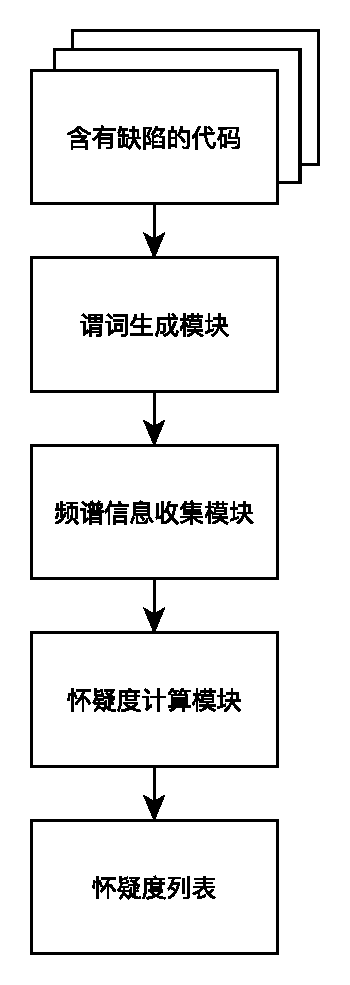
\includegraphics[width=5cm]{frame1} 
\caption{缺陷定位框架模块图} 
\label{fl_frame1}
\end{figure}

谓词生成模块生成预定义的谓词,或者利用机器学习模型预测出谓词。
频谱信息收集模块把生成的谓词插装到缺陷代码,执行测试用例,收集测试用例覆盖谓词真假分支的情况。
最后怀疑度计算模块利用频谱信息,带入公式中计算怀疑度。

具体的流程图如图\ref{fl_frame2}所示。下面将会具体讲述这些步骤的实现。

\begin{figure}[htbp] 
\centering 
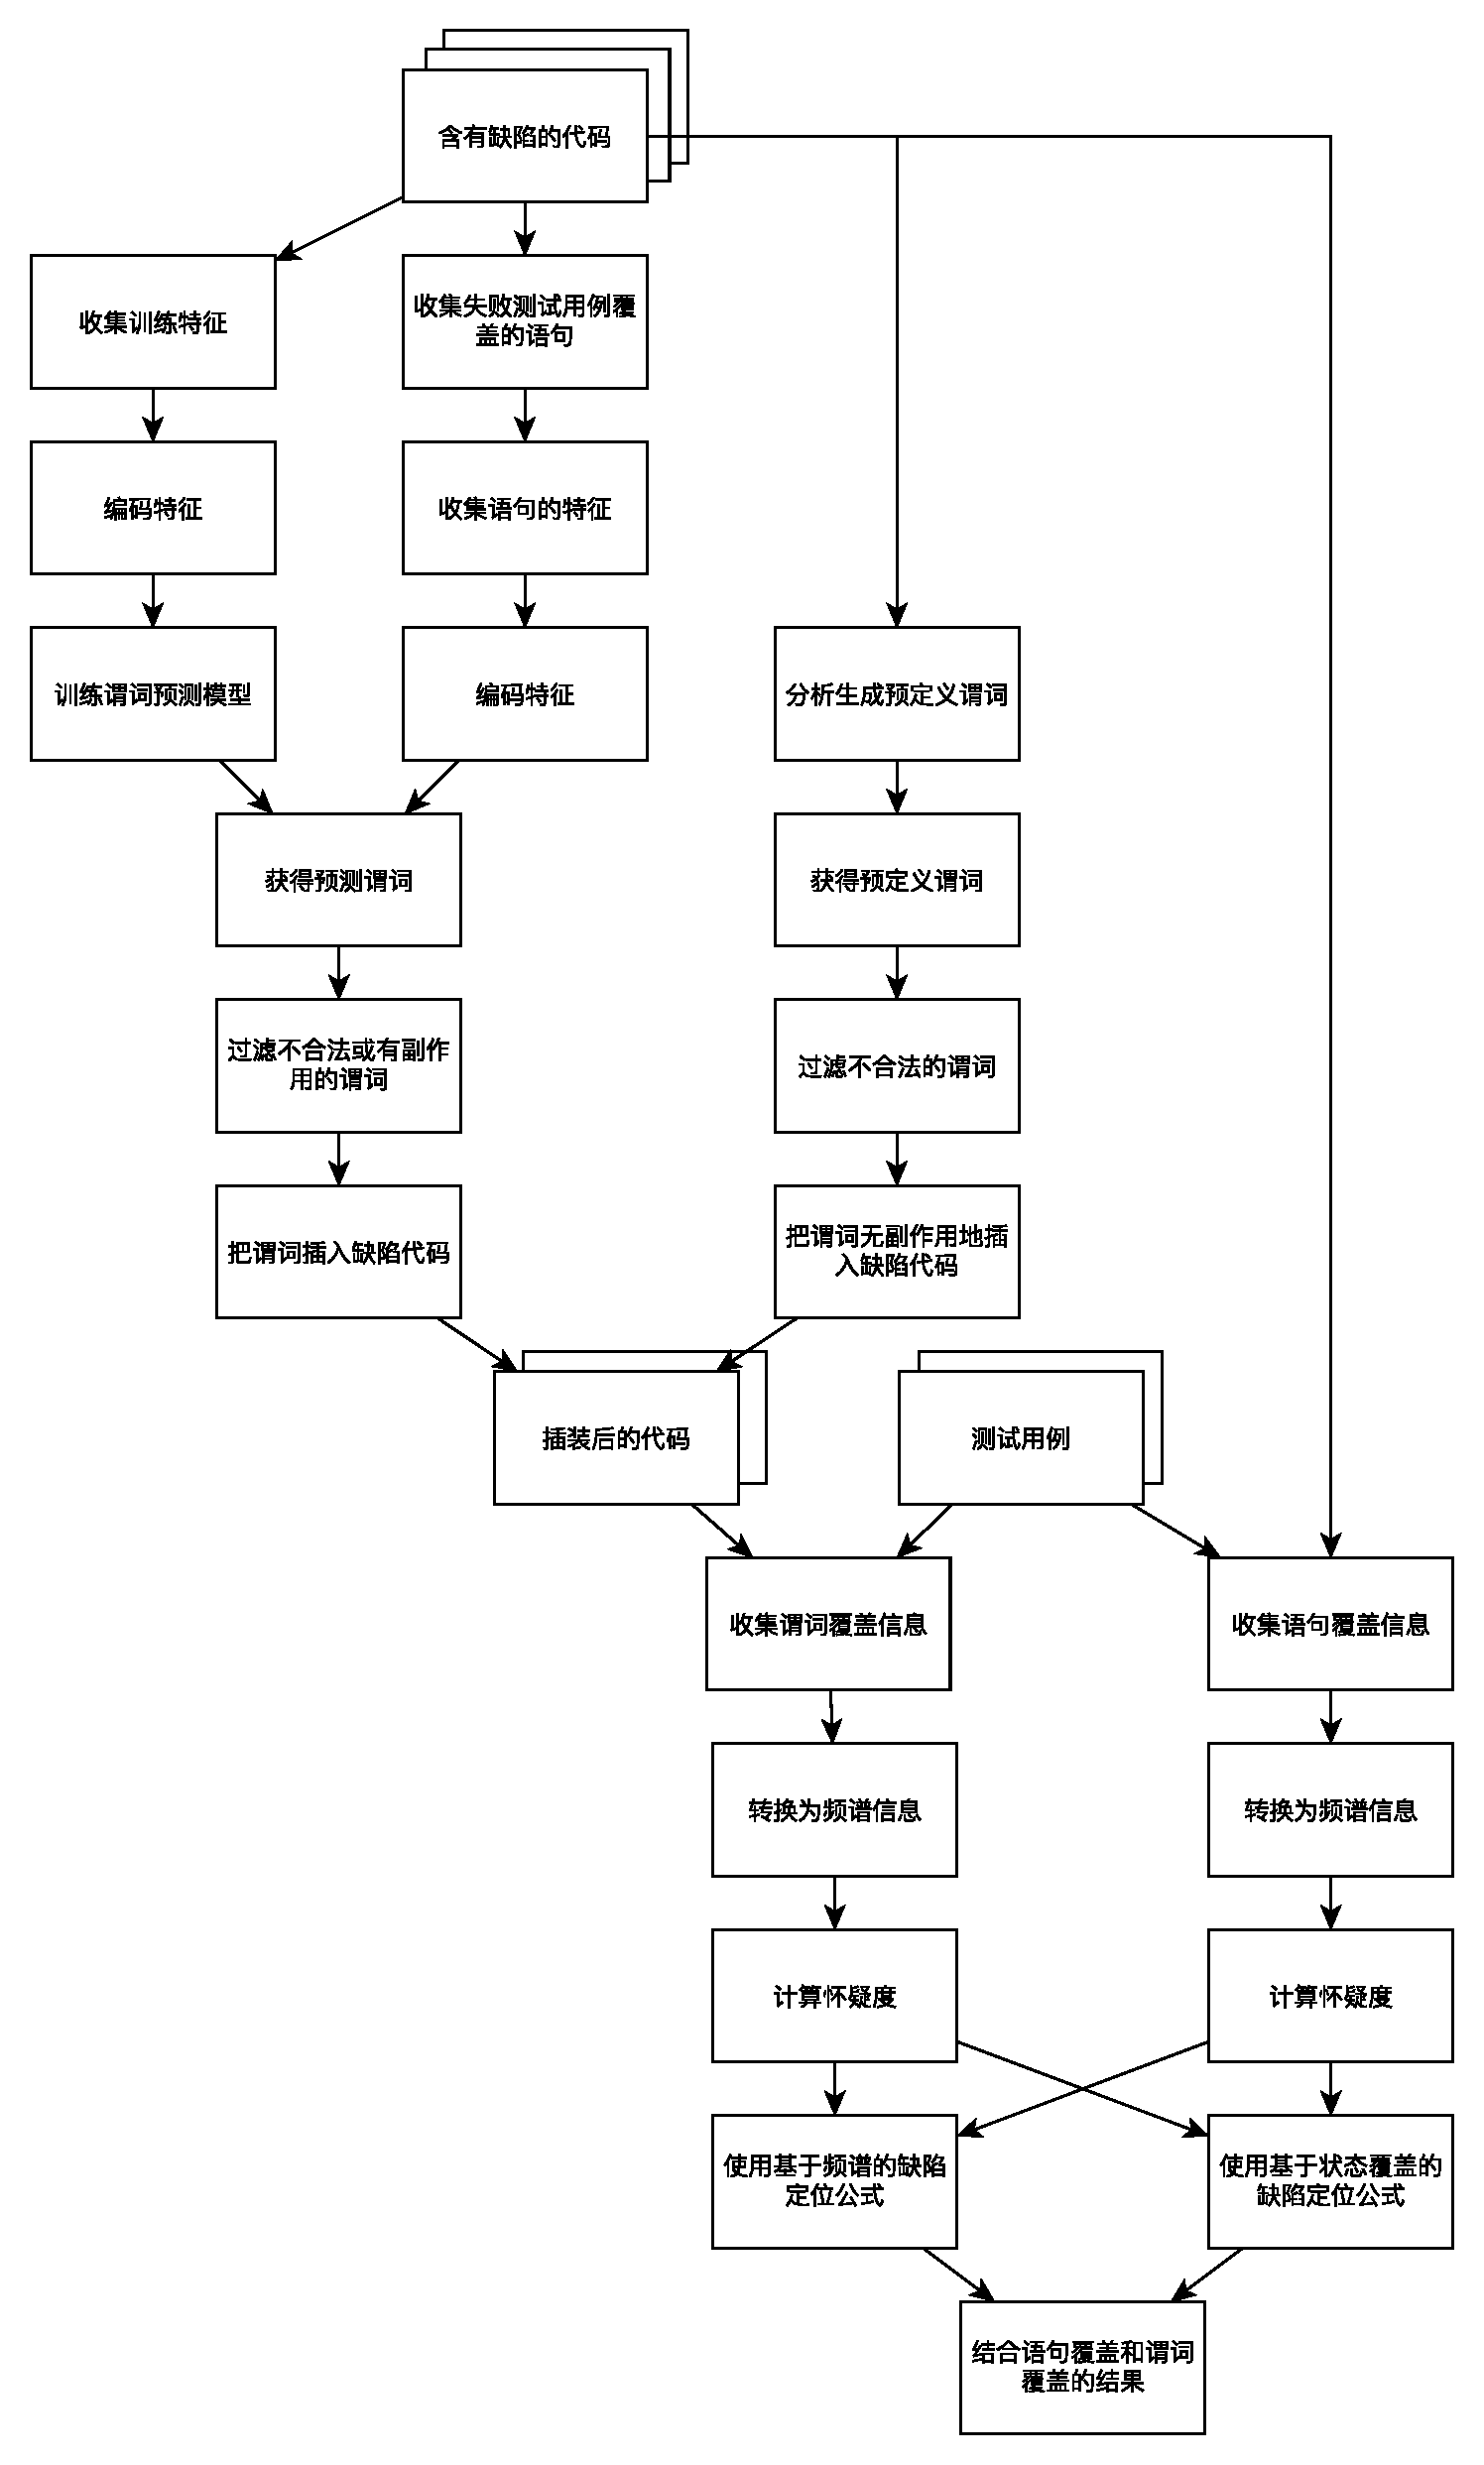
\includegraphics[width=13cm]{frame2} 
\caption{缺陷定位整体流程图}
\label{fl_frame2}
\end{figure}

\section{谓词生成模块}

谓词生成模块负责生成后续会使用的谓词.
谓词生成模块分为两种,一种是生成预测谓词,一种是生成预定义谓词。
生成谓词的语句都是被失败的测试用例覆盖的语句。

\subsection{生成预测谓词模块}

生成预测谓词使用的是机器学习模型,使用Java和Python实现。
首先,Java代码通过JDT遍历缺陷代码的抽象语法树,提取表\ref{var_feature}中的特征。
这些特征被写入到磁盘上的 csv 文件中。
Python程序则读入 csv 文件中的特征,对特征进行编码和训练。

编码阶段,先对变量名、文件名、函数名使用scikit-learn\footnote{\url{http://scikit-learn.org/}}的K-Means聚类,其值转为类编号。
聚类模型等被存储到磁盘。
使用 scikit-learn 的 \mycode{LabelEncoder} 对特征 FileName,MethodName,VarName,VarType,LastAssign,BodyUse
和 OutUse 进行编码,归一化为数字,然后使用 \mycode{OneHotEncoder} 转为独热编码。

训练阶段,特征被放入神经网络或者决策树中。
神经网络使用的全连接神经网络,用TensorFlow\footnote{\url{https://www.tensorflow.org/}}的 \mycode{DNNClassifier} 实现。
TensorFlow 是一个采用数据流图用于数值计算的开源软件库。
图中的节点表示数学操作,图中的线则表示在节点间相互联系的多维数据数组。
网络的输入使用 TensorFlow 的 \mycode{numpy\_input\_fn}。
使用这个函数的好处是,输入不需要在一开始的时候就被存储在内存,
而是在需要的时候才生成一个批(batch)的数据。
每次训练以一个批的数据为一次迭代。
VAR模型的网络会跑100个纪元(epoch),EXPR模型的网络会跑1000个纪元。
每一个纪元都会把整个输入数据遍历一次。
VAR模型和EXPR模型的批尺寸(batch size)都为128。
输入数据会被随机打乱(shuffle)。
训练使用 \mycode{DNNClassifier} 的 \mycode{train} 方法。
决策树使用 scikit-learn 中的决策树 \mycode{DecisionTreeClassfier} 。
训练使用其 \mycode{fit} 方法。
训练好的模型被保存在磁盘中。
神经网络模型直接通过设置 \mycode{model\_dir} 参数保存,
决策树模型使用 pickle\footnote{\url{https://docs.python.org/3/library/pickle.html}} 保存。

预测阶段,对收集的失败测试用例覆盖的语句进行谓词预测。
首先用Java的JDT提取语句中左值变量的特征,然后写入磁盘上的 csv 文件。
Python程序读入 csv 文件中的特征和编码阶段存储的聚类模型。
同时Python程序也会读入训练时使用的 csv 文件,以获取同样的 \mycode{LabelEncoder} 和 \mycode{OneHotEncoder}。
使用聚类模型对特征的变量名、函数名和文件名划入某个已有的分类。
然后用和训练时一样的 \mycode{LabelEncoder} 和 \mycode{OneHotEncoder} 对特征 FileName,MethodName,VarName,VarType,LastAssign,BodyUse
和 OutUse 进行编码。
最后把预测变量的特征传入训练好的VAR模型和EXPR模型中预测。
神经网络通过 \mycode{predict} 方法预测。
该方法返回预测结果的一个列表。
列表中一个元素对应于一个预测输入,该元素的 \mycode{probabilities} 域表示这个样本属于各个标签的概率,
\mycode{classes} 域表示表示这个样本的预测标签。
决策树通过 \mycode{predict\_proba} 方法预测,得到一个矩阵。每行对应一个样本,每列对应这个样本属于某个标签的概率。
VAR模型会输出这个变量出现在谓词中的概率,EXPR模型会对一个样本的概率值排序,取概率最高的200个输出。
最后,将同一个变量其VAR模型的输出$P_{var}$和EXPR模型的输出$P_{pred_i}$相乘,把联合概率大于$0.005$的变量及谓词输出。

验证阶段是在正常的缺陷定位中不存在的阶段。
在测试中被用于测试模型的预测准确性。
在验证阶段,输入数据会被使用 scikit-learn 的 \mycode{train\_test\_split} 函数随机分为70\%的训练集和30\%的验证集。
然后使用训练集去训练模型,对得到的模型使用验证集验证其准确率。
神经网络的准确率计算使用 \mycode{DNNClassifier} 自带的 \mycode{evaluate} 方法
的域 \mycode{accuracy} 获得。
决策树的准确率使用 \mycode{DecisionTreeClassfier} 自带的 \mycode{score} 方法获得。

过滤阶段,过滤掉预测出不合法或有副作用的谓词。
使用JDT遍历谓词过滤。
静态分析过滤后的谓词还会被单个编译过滤。
每条语句最终只有过滤后的五个概率最高的谓词和它们的相反谓词。

\subsection{生成预定义谓词模块}

生成预定义谓词使用Java的JDT遍历抽象语法树。

对于一个返回语句,只要其返回值不是空 \mycode{return;},就生成谓词。
对于条件语句 \mycode{if, for, while, do, switch},生成其条件表达式的谓词。
对于赋值语句和变量声明语句,如果其左值是基本数据类型,获取当前行可见的其他同类型变量,生成谓词。

预定义生成的谓词数量往往大于预测谓词的数量。
过滤的时候使用编译过滤速度较慢。
其实预定义谓词并不需要一一过滤。
首先,条件语句的谓词就是其条件表达式和其条件表达式取反,这种谓词肯定是编译正确的,所以不需要过滤。
对于返回语句来说,只要验证 \mycode{v > 0} 是否编译正确就可以知道 \mycode{v < 0} 等谓词是否编译正确。
对于数值对来说,只要验证 \mycode{a > b} 是否编译正确就可以知道 \mycode{a < b} 等谓词是否编译正确。
因此减少过滤的谓词数量。

\section{频谱信息收集模块} 

频谱信息收集模块主要分为两步,第一步是把谓词插入到代码中,第二步是执行测试用例收集执行信息。

插入谓词分为两种情况,一种是插入预测的谓词,一种是插入预定义的谓词。
插入预测的谓词采用普通的插入方法,而插入预定义的谓词采用无副作用的插入方法。
这两种方法都是使用JDT遍历抽象语法树,然后对函数声明 \mycode{MethodDeclaration} 节点进行一个对其字节点的递归遍历。
这是因为插入谓词涉及到修改语法树,因此对于一个要被修改的节点来说,其父节点是被需要的甚至也是要修改的。

插入预测谓词时直接插入即可。而插入预定义谓词时,可能会涉及到新建变量、修改原有语句等。
因为无副作用的插入方法会新建一个中间变量,然后用这个中间变量替换原有变量的位置。
比如,为了在 \mycode{return a.increase();} 处插入谓词 \mycode{a.increase() > 0},
首先是使用 \mycode{VariableDeclarationFragment} 新建一个变量,这个变量的变量名组成为
\mycode{"automatic\_" + lineNumber + "\_" + varCount}。
其中 \mycode{lineNumber} 是行号, \mycode{varCount} 是一个递增的新变量计数。
然后用这个 \mycode{VariableDeclarationFragment} 生成一个 \mycode{VarableDeclarationExpression} ,
得到 \mycode{int automatic\_11\_2}。
把这个 \mycode{VarableDeclarationExpression} 放入 \mycode{Assignment},得到 \mycode{int automatic\_11\_2 = a.increase();}。
把原本的返回语句改为 \mycode{return automatic\_11\_2;}。
然后谓词也要修改,
原本要插入的谓词是 \mycode{a.increase() > 0},
现在要插入的谓词应该是 \mycode{automatic\_11\_2 > 0}。

为了收集执行信息,需要在代码中加入一些计数、标记、打印的语句。
为了方便起见,这些方法被包装在一个负责收集这些信息的类的静态方法中,
而这个类会被放入到缺陷代码的源代码中。

在代码被插入谓词和记录频谱的语句后,使用测试用例执行代码。
频谱信息会被输出到文件中。
频谱信息分为两类,第一类是SOBER算法的频谱信息。
SOBER算法的每个谓词会对应若干个覆盖信息。
每一条覆盖信息对应一个测试用例的覆盖情况,包含三个数值,分别是谓词为真的次数、谓词为假的次数和当前测试用例是通过还是失败。
第二类是除SOBER以外的公式的频谱信息。
每个谓词对应一条覆盖信息,包含四个数值,分别是谓词真分支被覆盖的失败测试用例个数、谓词真分支被覆盖的通过测试用例个数、谓词(无论真假分支)被覆盖的失败测试用例个数和谓词(无论真假分支)被覆盖的通过测试用例个数。

除了收集谓词的覆盖情况外,还会收集语句的频谱信息,
包括语句被覆盖的失败测试用例个数和被覆盖的通过测试用例个数。

\section{怀疑度计算模块}

怀疑度计算模块根据频谱信息的不同也分为两种。
一种是SOBER算法的怀疑度计算,一种是其他算法的怀疑度计算。
在实现上,SOBER算法继承父类 \mycode{TrueFalseCoverageNumberAlgorithm} 抽象类,
其他算法继承父类 \mycode{PredicateCoverageAlgorithm} 抽象类。
子类需要实现两个函数,一个是 \mycode{getName} 返回算法名,
一个是 \mycode{getScore} 返回怀疑度。
父类负责从磁盘读取执行信息并处理为频谱信息,计算并结合语句的怀疑度和谓词怀疑度,根据怀疑度对语句进行排序,最后输出到磁盘。

在一条语句的多个谓词中,选择怀疑度最高的作为这个语句的最终谓词怀疑度。



	\chapter{实验与验证}

\section{研究问题}

本文提出了一个结合了基于频谱的缺陷定位和基于状态覆盖的缺陷定位的缺陷定位框架,
并且通过结合深入分析基于频谱的缺陷定位和基于状态覆盖的缺陷定位能够准确定位的原因。

本文试图回答以下几个问题:
\begin{enumerate}
\item \textbf{当使用不同的数据收集粒度时,缺陷定位技术的效果有什么不同?} \\
这个研究问题探索了数据收集的粒度对缺陷定位结果的影响。
本文主要考虑两种数据收集粒度,
第一种是谓词的数量,第二种是程序元素的大小。
具体来说,对于谓词数量,本文考虑不同谓词数量下的语句级别的缺陷定位效果的不同。
对于程序元素大小,本文考虑的是语句级别和方法级别的数据收集对缺陷定位效果的影响。
\item \textbf{不同的怀疑度计算公式会如何影响缺陷定位的结果?} \\
这个研究问题探索了缺陷定位公式的重要性,
并分析了是否还能通过改进缺陷定位公式去提升缺陷定位效果,
为后续研究提供了参考。
\item \textbf{缺陷定位技术的不同结合方式效果如何?} \\
在章\ref{sec:approach_comb}中,
本文探讨了 PREDSBFL 和COMBSD 两种结合缺陷定位技术的方法,
并且每种结合方法还有多种不同的结合方式。
这个研究问题研究了不同结合方式的效果。
\item \textbf{结合后的缺陷定位技术与现有技术相比,效果如何?} \\
在这个研究问题中,
本文提出的结合的缺陷定位技术将与现有技术进行比较,并对其结果进行分析。
\item \textbf{机器学习模型预测谓词的准确率如何?} \\
这个研究问题探索了谓词预测模型的准确率,
并且在不同的机器学习模型上进行了对比。
\item \textbf{机器学习模型预测的谓词能否帮助有效定位缺陷?} \\
这个研究问题比较了基于谓词预测的缺陷定位和本文提出的结合方法、现有方法之间的结果,
分析预测的谓词在定位缺陷中的作用和不足。
\end{enumerate}

\section{实验数据}

本文使用Defects4j数据集\parencite{Just2014Defects4J}(v1.0)作为实验对象,
下文所提到的Defects4j都是v1.0版本。
Defects4j数据集含有357个真实的缺陷,来自五个大型的开源软件项目,见表\ref{defects4j_details}。
其中,“实验缺陷数目”是本文在实验中实际使用了的缺陷数目,“代码行数(千行)”表示的是这五个项目最近的版本的代码行数。
本文只使用了330个缺陷是因为其余27个缺陷因为插装后的代码太大导致“code too large"的报错而无法运行。

\begin{table}
\centering
\begin{tabular}{|l|r|r|r|r|}
\hline
项目名称 & 缺陷数目 & 实验缺陷数目 & 代码行数(千行) & 测试用例数目 \\
\hline
JFree\textbf{Chart} & 26 & 26 & 96 & 2205 \\
\hline
\textbf{Closure} compiler & 133 & 122 & 90 & 7927 \\
\hline
Apache commons-\textbf{Math} & 106 & 98 & 85 & 3602 \\
\hline
Apache commons-\textbf{Lang} & 65 & 57 & 22 & 2245 \\
\hline
Joda-\textbf{Time} & 27 & 27 & 28 & 4130 \\
\hline
总计 & 357 & 330 & 321 & 20109 \\
\hline
\end{tabular}
\caption{Defects4j数据集缺陷情况}
\label{defects4j_details}
\end{table}

\section{实验标准}

为了验证本文提出的结合后的缺陷定位的效果,以及预测谓词的效果,
需要一套衡量缺陷定位效果的标准和预测谓词效果的标准。

\subsection{缺陷定位结果标准}

本文使用两种常用的缺陷定位标准: Top-k 的召回率和 EXAM 分数。

Top-k 的召回率衡量的是有多少缺陷能够排在怀疑列表的前k位。
根据Kochhar等人的研究\parencite{Kochhar2016Practitioners},
超过73\%的参与者认为观察怀疑列表的前5个程序元素是可以接受的,
几乎所有参与者都认为10个程序元素是可以接受的最大的需要观察的程序元素个数。
所以本文采用1,3,5,10作为k值。
对于怀疑度分数相同的程序元素,它们的排名会使用平均排名,这也是很多已有研究使用的方法\parencite{Pearson2017Evaluating,Xuan2014Learning,Steimann2013Threats,Wong2016A}。

EXAM 分数衡量是开发者需要查看多少个位置才能看到真正的缺陷。
$$
\mathrm{EXAM} = \frac{n}{N}
$$
其中$N$表示候选的程序元素个数(比如被失败的测试用例覆盖的语句),$n$表示缺陷程序元素排在怀疑度列表的第$n$位。
EXAM 分数是一个0到1之间的值,且值越小越好。
它反映出了含有缺陷的程序元素在所有可疑程序元素中的相对位置,
体现出整个缺陷定位方法的效果。
很多工作都使用了这个方法\parencite{Wong2012Effective,Pearson2017Evaluating}。

\subsection{谓词预测结果标准}

本文对谓词预测结果的评判方法采用机器学习分类问题的评判方法。

首先引入一些评估分类问题效果时需要的统计量。
混淆矩阵统计量见表\ref{confusion_matrix}。
样本总数为$N$。
正例反例为两个相对的概念。
对于多分类问题,其余分类都为反例。

\begin{table}
\centering
\begin{tabular}{|c|c|c|}
\hline
\multirow{2}*{真实情况} & \multicolumn{2}{|c|}{预测结果} \\
\cline{2-3}
~ & 正例 & 反例 \\
\hline
正例 & TP(真正例) & FN(假反例) \\
\hline
反例 & FP(假正例) & TN(真反例) \\
\hline
\end{tabular}
\caption{分类结果混淆矩阵}
\label{confusion_matrix}
\end{table}

准确率(accuracy)衡量的是分类正确的样本数占样本总数的比例:
$$
\mathrm{Accuracy} = \frac{TP + TN}{N} = \frac{TP + TN}{TP + FN + FP + TN}
$$
。

准确率能够衡量一个机器学习模型的预测情况,但是有的时候只有准确率还不够。
有的时候人们还关心查准率和召回率。

查准率(precision)衡量的是被分类为正例的样本中有多少是真的正例:
$$
\mathrm{Precision} = \frac{TP}{TP + FP}
$$。

查全率或召回率(recall)衡量的是正例中有多少被分类为正例:
$$
\mathrm{Recall} = \frac{TP}{TP + FN}
$$。

查准率和查全率是一对相互矛盾的度量。
一般来说,查准率高时,查全率低,而查准率低时,查全率高。
F1 度量结合查准率和查全率,给出一个便于比较的统一的值:
$$
\mathrm{F1} = \frac{2 \times \mathrm{Precision} \times \mathrm{Recall}}{\mathrm{Precision} + \mathrm{Recall}}
$$。

在本文的问题中,VAR模型是一个二分类模型,可以使用准确率、查准率、召回率和F1评判。
EXPR模型是一个多分类模型,而且分类数量往往是四位数,使用查准率和召回率会导致查准率和召回率数量非常大
(其数量和分类数量一致)。
所以本文对VAR模型使用准确率、查准率、召回率和F1标准,
而对EXPR模型只使用准确率标准。

\section{实验结果与分析}


	% 结论。
	\chapter{总结与未来工作}

本章对本文的工作进行总结,并且对未来的研究方向进行展望。

\section{总结}

本文结合了现有的缺陷定位技术,提出了结合现有缺陷定位技术的新的缺陷定位技术。
具体来说,
\begin{enumerate}
\item 本文提出了一种结合基于频谱的缺陷定位和基于状态覆盖的缺陷定位的方法~\textsc{LinPred}~,
并且在实际数据集 Defects4j 中与传统的基于频谱的缺陷定位和基于状态覆盖的缺陷定位进行了比较。
深入分析了基于频谱的缺陷定位和基于状态覆盖的缺陷定位起作用的原因,并且将其互补地结合起来。
可以发现\textsc{LinPred}在各个项目、各个公式上都有比较好的效果。
\item 本文提出了一种基于机器学习的预测谓词模型,来完善基于状态覆盖的缺陷定位中的预定义谓词。
实验效果发现,随机森林模型预测出的谓词的EXAM值比预定义谓词更优,
而神经网络模型预测出的谓词的Top-1值与预定义谓词相当。
预定义谓词与预测谓词具有互补性,两者结合后效果进一步提升。
\end{enumerate}

本文发现:
\begin{enumerate}
\item 更细粒度的数据收集会让缺陷定位效果变好。
\item 在Defects4j数据集中基于频谱的缺陷定位公式的效果优于基于状态覆盖的缺陷定位公式效果。
\item 在预定义谓词中,分支谓词对\textsc{LinPred}效果提升最明显。
本质上与使用分支覆盖的基于频谱的缺陷定位技术相同。
\item 预测谓词能够帮助更好地定位缺陷,与预定义谓词结合后效果更佳。
\end{enumerate}

\section{未来工作}

本文尝试了多种怀疑度计算公式。
统计性调试在 Defects4j 项目上效果不佳,但是并不能认为这个公式效果不好。
只是因为统计性调试不适用于失败测试用例少的场景。
所以可以考虑针对不同的应用场景,自动使用不同的怀疑度公式。
将每一个怀疑度公式的作用发挥到最好。

本文发现分支谓词起对定位缺陷起了重要作用。
同时发现了高频的预测谓词往往是和空指针的比较,和常数的比较。
可见某些类型的谓词具有更好的甄别缺陷的能力。
但是预测谓词的范围受限于项目中出现的条件表达式,
所以可能还有很多种具有明显甄别意义的谓词没有考虑到。
可以考虑增加可预测谓词的种类,来更好定位缺陷。

本文中,预测谓词取得了比较好的效果。
但是预测谓词仍有较大的提升空间,尤其是EXPR模型的准确率仍然较低。
在以后的工作中,可以考虑加入更多的特征、采样点,来提升准确率。
或者,可以考虑从另一些方面来建立模型。
比如在章\ref{sec:eval_pref_predict}中,曾经考虑过谓词是否具有积极影响。
可以尝试建立一个分类器,其分类目标是一个谓词是否具有积极影响。


	% 正文中的附录部分。
	\appendix
	% 排版参考文献列表。bibintoc 选项使“参考文献”出现在目录中;
	% 如果同时要使参考文献列表参与章节编号,可将“bibintoc”改为“bibnumbered”。
	\printbibliography[heading = bibintoc]
	% \bibliographystyle{IEEEtran}%

	% \bibliography{thesis.bib}
	% 各附录。
	% \include{chap/encl1}

	% 以下为正文之后的部分,默认不进行章节编号。
	\backmatter
	% 致谢。
	\chapter{致谢}

感谢北京大学和北京大学软件工程所,让我能够接触到前沿的科研项目。
浓厚的学术氛围感染了我,敦促我不断学习,打下了科研的坚实基础。

感谢熊英飞研究员,张路教授和郝丹副教授对我的指导。
我从大三开始就在张路老师的小组里学习,近五年的时间里三位老师对我耐心地指导和帮助,让我受益颇多。
从最开始的浮点数计算误差相关的研究,到自动缺陷定位的研究,
我从一个初出茅庐的计算机专业低年级学生,
变成了一个能够完成很多艰难计算机任务的高年级研究生。
老师们的培养让我在计算机基础知识,代码能力,科研能力等方面都有提升。
我也在熊英飞研究和张路教授的指导下发表了两篇CCF-A类的论文,一篇第一作者,一篇第二作者。

感谢姜佳君同学,和我一起讨论、完成这个研究。
他提出了许多宝贵的想法与建议,并且与我一起实现了\textsc{LinSD}。

感谢王博同学和臧琳飞师姐,他们的基于机器学习的缺陷修复给了本文非常多的帮助。
本文使用的从Java代码中提取特征的JDT代码来自于他们的基于机器学习的缺陷修复的代码。

最后,感谢我的父母一直陪伴着我、支持着我。他们一直是我坚强的后盾。
	% 原创性声明和使用授权说明。
	\include{chap/originauth}
\end{document}

% vim:ts=4:sw=4
